\section{Appendix}

\subsection{Detailed Derivation of the Planning Module}\label{app:planning_derivation}
\RE{
    In this section, we provide a detailed derivation of the planning module. By approximating the $Q(z)$ with $Q(z|a, q, \gG)$, the KL divergence can be calculated as
    \begin{equation}
        \label{eq:kl_full}
        \begin{aligned}
            \gL_{\text{plan}} =\KL(Q(z)\Vert P_\theta(z|q)) & = \KL(Q(z|a, q, \gG)\Vert P_\theta(z|q)),                            \\
                                                            & = \E_{z\sim Q(z|a, q, \gG)}[\log Q(z|a, q, \gG)-\log P_\theta(z|q)], \\
                                                            & = -\E_{z\sim Q(z|a, q, \gG)}\log P_\theta(z|q) + \text{CONST},
            % &= \RE{- \sum_{z\in\gZ^*} Q(z|a, q, \gG) \log P_\theta(z|q) + \text{CONST},} \\
            % &= \RE{- \frac{1}{|\gZ^*|}\sum_{z\in\gZ^*} \log P_\theta(z|q),}
        \end{aligned}
    \end{equation}
    where the expectations cannot be computed exactly because of the large number of valid relation paths $\gZ$, so we approximate it by using the shortest paths $z\in\gZ^*\subset\gZ$ between $e_q$ and $e_a$ in KGs \citep{zhang2022subgraph}. This can be formulated as
    \begin{equation}
        \label{eq:kl_approx}
        \gL_{\text{plan}} = - \sum_{z\in\gZ^*} Q(z|a, q, \gG) \log P_\theta(z|q) + \text{CONST}.
    \end{equation}
    Based on \eqref{eq:posterior}, by assuming a uniform distribution over the set of shortest paths $\gZ^*$, we can rewrite the \eqref{eq:kl_approx} as
    \begin{equation}
        \label{eq:kl_uniform}
        \gL_{\text{plan}} = - \frac{1}{|\gZ^*|}\sum_{z\in\gZ^*} \log P_\theta(z|q) + \text{CONST},
    \end{equation}
    where the $\text{CONST}$ is omitted in the final optimization since it makes no contributions to the loss.
}
\subsection{Detailed Related Work}

\subsubsection{LLM Reasoning Prompt}

Many studies have been proposed to harness the reasoning ability of LLMs to handle complex tasks through prompting \citep{wei2022chain,wang2022self,yao2023tree,besta2023graph,pan2023integrating,zheng2023large,jin2023time,jin2024position}. Chain-of-Thought \citep{wei2022chain} enables LLMs to generate a reasoning chain that could be helpful to reasoning. Tree of thoughts \citep{yao2023tree} expands the reasoning chain to a tree structure to explore more reasoning paths. Graph of thoughts \citep{besta2023graph} further models the reasoning chain as a graph with an aggregation operation to synergize the reasoning paths.
Plan-and-solve \citep{wang2023plan} prompts LLMs to generate a plan and execute based on it. DecomP \citep{he2021improving} prompts LLMs to decompose the reasoning task into a series of sub-tasks and solve them step by step. However, the problem of hallucinations and lack of knowledge affect the faithfulness of the reasoning. ReACT \citep{yao2022react} treats LLMs as agents, which interact with the environment to get the latest knowledge for reasoning. To explore faithful reasoning, Entailer \citep{tafjord2022entailer} introduces a verifier to validate the reasoning steps generated by LLMs. \citet{creswell2022faithful} present a framework including two LLMs that are used for selecting and generating reasoning steps, respectively.
FAME \citep{hong2023faithful} introduces the Monte-Carlo planning to generate faithful reasoning steps. RR \citep{he2022rethinking} and KD-CoT \cite{wang2023knowledge} aim to retrieve relevant knowledge from KGs to produce faithful reasoning plans for LLMs. Think-on-Graph \citep{sun2024thinkongraph} and KG-Agent \citep{jiang2024kg} treat LLMs as agents to interact with KGs via prompting to get the latest knowledge for reasoning.


\subsubsection{Knowledge Graph Question Answering}
Knowledge graphs contain abundant factual knowledge in a structured format, which has attracted great attention from researchers \citep{zheng2022multi,zheng2023towards,pan2023integrating,Liangke_SymCLKG_TKDE}. Knowledge graph reasoning aims to derive new insights based on the existing graph structure and facts \citep{Liangke_Survey,wang2023survey,luo2023npfkgc,zhao2023towards}. Graph neural networks that effectively capture the structure information have also been widely used in KG reasoning \cite{zheng2022rethinking,zheng2023finding,zheng2023gnnevaluator,zheng2023structure,liu2023learning,liu2024towards}.
%
As a typical reasoning task, knowledge graph question answering (KGQA) aims to obtain answers based on knowledge from KGs, which can be generally divided into three categories: 1) embedding-based methods, 2) retrieval-augmented methods, and 3) semantic parsing methods.

\textbf{Embedding-based methods} model the entities and relations in embedding space and design special model architectures to reason answers. KV-Mem \citep{miller2016key} adopts a Key-Value memory network to store triples for reasoning. EmbedKGQA \citep{saxena2020improving} and NSM \citep{he2021improving} utilize the sequential model to mimic the multi-hop reasoning process. QA-GNN \citep{yasunaga2021qa} and Greaselm \citep{zhang2021greaselm} further adopt the graph neural network to capture the graph structure for reasoning. However, these methods need to design different model architectures, which are not flexible and generalizable.

\textbf{Retrieval-augmented methods} aims to retrieve the relative facts from the KGs to improve the reasoning performance. Early works adopt the page rank or random walk algorithm to retrieve subgraphs from KGs for reasoning \citep{sun2018open, sun2019pullnet}. However, they ignore the semantic information in questions and lead to noisy retrieval results. \citet{zhang2022subgraph} proposes a relation paths-based subgraph retrieval, resulting a better retrieval and QA performance. Other lines of studies retrieving triples from KGs via BM25 \citep{li2023graph} or DPR \citep{karpukhin2020dense, yu2022kg} to improve the performance of LLMs. They discard the structure information in KGs which leads to suboptimal results. Recently, UniKGQA \citep{jiang2022unikgqa} unifies the graph retrieval and reasoning process into a single model with LLMs, which achieves state-of-the-art performance on KGQA tasks.

\textbf{Semantic parsing methods} parse the question into a structural query (e.g., SPARQL) which can be executed by a query engine to get answers \citep{sun2020sparqa,lan2020query}. ArcaneQA \citep{gu2022arcaneqa} dynamically generates the query based on results from previous steps. RnG-KBQA \citep{ye2022rng} first enumerate all possible queries and then rank them to get the final output. These methods heavily rely on the quality of generated queries. If the query is not executable, no answers will be generated. DECAF \citep{yu2022decaf} combines semantic parsing and LLMs reasoning to jointly generate answers, which also reach salient performance on KGQA tasks.

\subsection{Retrieval Algorithm}\label{app:retrieval}
Given a question $q$ and a relation path as plan $z$, we adopt a constrained breadth-first search to retrieve the reasoning paths. The pseudocode code is presented in \Cref{alg:retrieval}.

We first initialize a queue of current reasoning paths $\gQ$ with the entities in the question $\gT_q$ (line 3-5). Then, we iteratively expand each reasoning path in $\gQ$ by adding the triples that are connected to the entities in the queue following the relation in relation path (line 11-19). The reasoning path is expanded until the length is equal to the length of the relation path. The expanded reasoning path is added to the set $\gW_z$ as the final results (line 8-10).

\begin{algorithm}
    \caption{Retrieve reasoning paths based on relation paths}\label{alg:retrieval}
    \KwIn{Question $q$, relation path $z=\{r_1,r_2,\dots,r_l\}$, KG $\gG$.}
    \KwOut{Reasoning paths $\gW_z$.}

    $\gW_z \gets \emptyset$\;
    $\gQ \gets \text{Queue()}$\;
    \ForEach{$e_q \in \gT_q$}{
    $\gQ.\text{append}((e_q, []))$; \tcp{Initialize queue with question entities.}
        }
        % \While{\gQ \neq \empty}{while block}
        \While{$\gQ \neq \emptyset$}{
    $(s, w_z) \leftarrow \gQ.\text{pop}()$\;
        \If{$\text{len}(w_z) = \text{len}(z)$}{
            $\gW_z.\text{append}(w_z)$\;
        }
        \If{$\text{len}(w_z)< \text{len}(z)$}{
    $r \gets z[\text{len}(w_z) + 1]$; \tcp{Get relation for next step.}
    \ForEach{$(s,r',t)\in\gG$}{
        \If{$r' = r$}{
            $w'_z.\text{append}((s,r,t))$; \tcp{Expand the reasoning path.}
            $\gQ.\text{append}((t, w'_z))$\;
            }
            }
        }
    }

    \Return{$\gW_z$.}\;

\end{algorithm}

% \begin{wraptable}{r}{.35\columnwidth}
\begin{table}[]
    \centering
    % \vspace{-3mm}
    \caption{Statistics of datasets.}
    \label{tab:dataset}
    % \resizebox{.35\columnwidth}{!}{%
    \begin{tabular}{@{}c|ccc@{}}
        \toprule
        Datasets & \#Train & \#Test & Max \#hop \\ \midrule
        WebQSP   & 2,826   & 1,628  & 2         \\
        CWQ      & 27,639  & 3,531  & 4         \\ \bottomrule
    \end{tabular}%
    % }
    % \vspace{-3mm}
% \end{wraptable} 
\end{table}

\begin{table}[]
    \centering
    \caption{Statistics of the number of answers for questions in WebQSP and CWQ.}
    \label{tab:ans_dist}
    %\resizebox{\textwidth}{!}{%
    \begin{tabular}{@{}ccccc@{}}
        \toprule
        Dataset & \#Ans = 1 & 2 $\geq$ \#Ans $\leq$ 4 & 5 $\geq$ \#Ans $\leq$ 9 & \#Ans $\geq$ 10 \\ \midrule
        WebQSP  & 51.2\%    & 27.4\%                  & 8.3\%                   & 12.1\%          \\
        CWQ     & 70.6\%    & 19.4\%                  & 6\%                     & 4\%             \\ \bottomrule
    \end{tabular}%

\end{table}

\begin{table}[]
    \centering
    \caption{Statistics of the question hops in WebQSP and CWQ.}
    \label{tab:hop_dist}
    %\resizebox{\textwidth}{!}{%
    \begin{tabular}{@{}cccc@{}}
        \toprule
        Dataset & 1 hop                         & 2 hop   & $\geq$ 3 hop \\ \midrule
        WebQSP  & 65.49                      \% & 34.51\% & 0.00\%       \\
        CWQ     & 40.91                      \% & 38.34\% & 20.75\%      \\ \bottomrule
    \end{tabular}%
    %}
\end{table}

\begin{table}[]
    \centering
    \caption{Statistics of MetaQA-3hop datasets.}
    \label{tab:metaqa}
    %\resizebox{2in}{!}{%
    \begin{tabular}{@{}c|ccc@{}}
        \toprule
        Datasets    & \#Train & \#Test & \#hop \\ \midrule
        MetaQA-3hop & 1,000   & 1,4274 & 3     \\\bottomrule
    \end{tabular}%
\end{table}

\subsection{Datasets}\label{app:dataset}
We adopt two benchmark KGQA datasets: WebQuestionSP (WebQSP)\footnote{\url{https://www.microsoft.com/en-us/download/details.aspx?id=52763}} \citep{yih2016value} and Complex WebQuestions (CWQ)\footnote{\url{https://www.tau-nlp.sites.tau.ac.il/compwebq}} \citep{talmor2018web} in this work. We follow previous works \citep{sun2018open,jiang2022unikgqa} to use the same train and test splits for fair comparison. The statistic of the datasets are given in \Cref{tab:dataset}. The statistics of the answer numbers and reasoning hops are presented in \Cref{tab:ans_dist} and \Cref{tab:hop_dist}, respectively.

% \noindent\textbf{WebQuestionSP (WebQSP)} contains 4,737 different questions and requires up to 2-hop reasoning. Questions in WebQSP have up to 10 answers annotated. 

% \noindent\textbf{Complex WebQuestions (CWQ)} is a more complex datasets, which contains 34,689 different questions and requires up to 4-hop reasoning. Questions in CWQ also have up to 10 answers annotated.

To evaluate the transferability of \ourmethod to other KGs. We further select the MetaQA-3hop dataset \citep{zhang2018variational} which is based on Wiki-Movies KGs\footnote{\url{https://research.fb.com/downloads/babi}}. We select 1000 samples from the training split. The statistic of the dataset is presented in \Cref{tab:metaqa}.

Both WebQSP and CWQ can be reasoned based on Freebase KGs\footnote{\url{https://github.com/microsoft/FastRDFStore}} \citep{bollacker2008freebase}. To reduce the size of KGs, following previous works \citep{he2021improving,jiang2022unikgqa}, we construct a subgraph of Freebase by extracting all triples that contain within the max reasoning hops of question entities in WebQSP and CWQ. Similarly, we construct a subgraph of Wiki-Movies KGs for MetaQA-3hop. The statistics of constructed KGs are presented in \Cref{tab:kg}.

We construct the instruction-tuning dataset using the training split of WebQSP and CWQ datasets. For planning optimization, we generate data by extracting the shortest paths that connect the questions and answers, which serve as supervisory signals. In the retrieval-reasoning optimization phase, we feed both extracted shortest paths together with the questions to predict the answers. To enhance interpretability, we randomly select 1000 samples from each dataset along with their reasoning paths and answers. These are then input into ChatGPT to produce interpretive responses, which help empower our method in generating results with good explainability. The statistics of final training datasets are shown in \Cref{tab:it-data}.

\begin{table}[]
    \centering
    \caption{Statistics of constructed knowledge graphs.}
    \label{tab:kg}
    %\resizebox{\textwidth}{!}{%
    \begin{tabular}{@{}cccc@{}}
        \toprule
        KG         & \#Entities & \#Relations & \#Triples \\\midrule
        Freebase   & 2,566,291
                   & 7,058      & 8,309,195               \\
        Wiki-Movie & 43,234     & 9           & 133,582   \\

        \bottomrule
    \end{tabular}%
    %}
\end{table}

\begin{table}[]
    \centering
    \caption{The statistics of the instances in the instruction-tuning datasets.}
    \label{tab:it-data}
    % \resizebox{\columnwidth}{!}{%
    \begin{tabular}{@{}ccc@{}}
        \toprule
        Planing Data & Retrieval-reasoning Data & Interpretability Data \\ \midrule
        216,006      & 30,465                   & 2,000                 \\ \bottomrule
    \end{tabular}%
    % }
\end{table}


\subsection{Baselines}\label{app:baselines}


We compare \ourmethod with 21 baselines grouping into 5 categories: 1) \emph{Embedding-based methods}, 2) \emph{Retrieval-augmented methods}, 3) \emph{Semantic parsing methods}, 4) \emph{LLMs}, and 5) \emph{LLMs+KGs methods}. The details of each baseline are described as follows.

\noindent\textbf{Embedding-based methods.}
\begin{itemize}
    \item KV-Mem \citep{miller2016key} adopts a Key-Value memory network to store triples and perform multi-hop reasoning by iterative operating on the memory.
    \item EmbedKGQA \citep{saxena2020improving} models the reasoning on KGs as a sequential link prediction problem by using the embedding of entities and questions.
    \item NSM \citep{he2021improving} utilizes the sequential model to mimic the multi-hop reasoning process.
    \item TransferNet \citep{shi2021transfernet} adopts a graph neural network to capture the relevance between entities and questions for reasoning.
    \item KGT5 \citep{saxena2022sequence} finetunes a sequence-to-sequence framework on KGs and generates answers based on the input question.
\end{itemize}

\noindent\textbf{Retrieval-augmented methods.}
\begin{itemize}
    \item GraftNet \citep{sun2018open} retrieves relevant subgraphs from KGs with entity linking.
    \item PullNet \citep{sun2019pullnet} trains a retrieval model composed of a LSTM and a graph neural network to retrieve a question-specific subgraph.
    \item SR+NSM \citep{zhang2022subgraph} proposes a relation-path retrieval to retrieve subgraphs for multi-hop reasoning.
    \item SR+NSM+E2E \citep{zhang2022subgraph} further adopts an end-to-end training strategy to jointly train the retrieval and reasoning modules of SR+NSM.
\end{itemize}

\noindent\textbf{Semantic parsing methods.}
\begin{itemize}
    \item SPARQL \citep{sun2020sparqa} presents a novel skeleton grammar to represent the high-level structure of a complex question with language modes.
    \item QGG \citep{lan2020query} generates a query graph for a question by simultaneously adding constraints and extending relation paths.
    \item ArcaneQA \citep{gu2022arcaneqa} dynamically generates the query based on results from previous steps.
    \item RnG-KBQA \citep{ye2022rng} first enumerates all possible queries and then ranks them to get the final output.
\end{itemize}

\noindent\textbf{Large language models (LLMs).}
\begin{itemize}
    \item Flan-T5 \citep{chung2022scaling} is an enhanced version of T5 models that is instruction finetuned on mixture of tasks.
    \item Alpaca \citep{taoristanford} is based on LLaMA and finetuned on an instruction-following dataset.
    \item LLaMA2-Chat \citep{touvron2023llama} is a large language model that is optimized for dialogue purposes.
    \item ChatGPT\footnote{\url{https://openai.com/blog/chatgpt}} is a powerful closed-source LLM that could follow instructions to conduct complex tasks\footnote{\RE{Experiments are conducted with the ChatGPT model released between July. to Sept., 2023.}}.
    \item ChatGPT+CoT \citep{wei2022chain} uses the Chain-of-thought prompt to improve the reason ability of ChatGPT.
\end{itemize}

\noindent\textbf{LLMs+KGs methods.}
\begin{itemize}
    \item KD-CoT \cite{wang2023knowledge} retrieves relevant knowledge from KGs to generate faithful reasoning plans for LLMs.
    \item UniKGQA \citep{jiang2022unikgqa} unifies the graph retrieval and reasoning process into a single model with LLMs, which achieves state-of-the-art performance on KGQA tasks.
    \item DECAF \citep{yu2022decaf} combines semantic parsing and LLMs reasoning to jointly generate answers, which also reach salient performance on KGQA tasks.
\end{itemize}

\subsection{Implementation Settings}\label{app:settings}
For \ourmethod, we use LLaMA2-Chat-7B \citep{touvron2023llama} as the LLM backbone, which is instruction finetuned on the training split of WebQSP and CWQ as well as Freebase for 3 epochs. The batch size is set to 4 and the learning rate is set to 2e-5. We use the cosine learning rate scheduler policy with the warmup ratio set to 0.03. The training is conducted on 2 A100-80G GPUs for 38 hours. During inference, we first adopt the LLM to generate top-$K$ relation paths with the highest probability as the plans. Then, we adopt the \Cref{alg:retrieval} to retrieve reasoning paths, which are fed into the LLM to reason the final answers.

For LLM beelines, we use zero-shot prompting to conduct KGQA, which directly asks LLMs to answer the question. For other baselines, we directly copy their results reported in UniKGQA \citep{jiang2022unikgqa} and DECAF \citep{yu2022decaf} for comparisons.

\RE{For combining the planning module of \ourmethod with different LLMs, we use the planning module to generate plans (relation paths), which are executed on KGs to retrieve the reasoning paths. The retrieved paths are fed into different LLMs during inference by utilizing the reasoning prompts template shown in \Cref{app:prompts}.}

\subsection{Additional Experiment Results}

\begin{table}
    \centering
    \caption{Performance of \ourmethod on MetaQA-3hop.}
    \label{tab:transfer}
    %\resizebox{2.2in}{!}{%
    \begin{tabular}{@{}l|cc@{}}
        \toprule
        \multirow{3}{*}{Strategies}         & \multicolumn{2}{c}{MetaQA-3hop}                  \\ \cmidrule(l){2-3}
                                            & Hits@1                          & F1             \\ \midrule
        \ourmethod (train from scratch)  & 84.81                           & 41.32          \\
        \ourmethod (transfer from Freebase) & \textbf{88.98}                  & \textbf{50.68} \\ \bottomrule
    \end{tabular}
    %}
\end{table} 


\begin{table}
    \centering
    \RE{
    \caption{Training time comparison.}
    \label{tab:time}
    %\resizebox{2.2in}{!}{%
    \begin{tabular}{@{}c|cc@{}}
        \toprule
        Method & Training on Freebase & Transferring to Wiki-Movies \\
        \midrule
        \ourmethod & 38 hours & 2 hours \\
        \bottomrule
    \end{tabular}
    %}
    }
\end{table} 
\subsubsection{Transferability to Other KGs}
We evaluate the transferability of \ourmethod to other KGs. We select the MetaQA-3hop dataset \citep{zhang2018variational} which is based on Wiki-Movies KGs. We select 1000 samples from the training split and utilize two training strategies to finetune \ourmethod: 1) \emph{training from scratch}, where we directly train \ourmethod from LLaMA2-Chat with 1000 samples; 2) \emph{transfer from Freebase}, where we conduct a further finetuning based on \ourmethod trained for Freebase. The results are shown in \Cref{tab:transfer}. From results, we can see that transfer from Freebase achieves better performance than training from scratch, which demonstrates the transferability of \ourmethod to other KGs.

\RE{We also compare the training time on Freebase and transferring to Wiki-Movies KGs. From results shown in \Cref{tab:time}, we can see that the training time on Freebase is 38 hours, while the transferring time is only 2 hours. This demonstrates the efficiency of transferring \ourmethod to other KGs.}



\begin{table}[]
    \centering
    \caption{Performance on WebQSP with different training data.}
    \label{tab:webqsp_only}
    %\resizebox{\columnwidth}{!}{%
    \RE{
        \begin{tabular}{@{}cccc@{}}
            \toprule
            Method     & Training Data & Hits@1 & F1   \\ \midrule
            UniKGQA    & WebQSP        & 77.2   & 72,2 \\
            \ourmethod & WebQSP        & 81.5   & 61.8 \\
            \ourmethod & WebQSP+CWQ    & 85.7   & 70.8 \\ \bottomrule
        \end{tabular}%
        %}
    }
\end{table}

\begin{table}[]
    \centering
    \caption{Performance on CWQ with different training data.}
    \label{tab:cwq_only}
    %\resizebox{\columnwidth}{!}{%
    \RE{
        \begin{tabular}{@{}cccc@{}}
            \toprule
            Method     & Training Data & Hits@1 & F1   \\ \midrule
            UniKGQA    & CWQ           & 51.2   & 49.1 \\
            \ourmethod & CWQ           & 59.1   & 52.9 \\
            \ourmethod & WebQSP+CWQ    & 62.6   & 56.2 \\ \bottomrule
        \end{tabular}%
        %}
    }
\end{table}

\subsubsection{Performance with Different Training Data}
\RE{
    In our experiment, we finetune \ourmethod jointly on the training set of both WebQSP and CWQ datasets to maximize the ability of \ourmethod for reasoning on Freebase. To fairly compare with other methods (e.g., UniKGQA \citep{jiang2022unikgqa}) that are only trained on single dataset, we provide additional results of the performance of \ourmethod trained on single dataset. From the results shown in \Cref{tab:webqsp_only,tab:cwq_only},  we can see that \ourmethod trained on single dataset still outperforms the STOA baselines (UniKGQA). Besides, we can also find that jointly training \ourmethod on multiple datasets can further improve the performance. In the future, we will try to generate more QA datasets from Freebase to further improved the reasoning ability of \ourmethod.
}


\subsubsection{Performance Comparison with Different Finetuned LLMs}
\RE{
    In \Cref{tab:kgqa}, we report the zero-shot performance of different LLMs. However, \ourmethod is finetuned on the training split of the QA dataset. To make a fair comparison, we further report the performance of the LLMs finetuned on the training split of the QA dataset in \Cref{tab:ft_llm}. From the results, we can see that \ourmethod still outperforms the finetuned LLMs.
}
\begin{table}[]
    \centering
    \caption{Performance comparison with different finetuned LLMs (Hits@1).}
    \label{tab:ft_llm}
    \RE{
    %\resizebox{\columnwidth}{!}{%
    \begin{tabular}{@{}ccc@{}}
    \toprule
    Method                      & WebQSP         & CWQ            \\ \midrule
    Alpaca-7B (Zero Shot)      & 51.78          & 27.44          \\
    LLaMA2-Chat-7B (Zero Shot) & 64.37          & 34.60          \\
    Alpaca-7B (Finetuned)       & 74.57          & 55.98          \\
    LLaMA2-Chat-7B (Finetuned)  & 73.89          & 53.49          \\\midrule
    \ourmethod                  & \textbf{85.75} & \textbf{62.65} \\ \bottomrule
    \end{tabular}%
    }
\end{table}

\subsubsection{Retrieval Costs}\label{app:retrieval_cost}

We present the retrieval time and number of retrieved reasoning paths in \Cref{fig:retrieval_cost}. From results, we can see that the retrieval time increases with the number of top-$K$ relation paths. Therefore, we should select a proper $K$ to balance the retrieval time and the number of retrieved reasoning paths. In experiments, we set $K=3$.

\begin{figure}[]
    \begin{center}
        %\framebox[4.0in]{$\;$}
        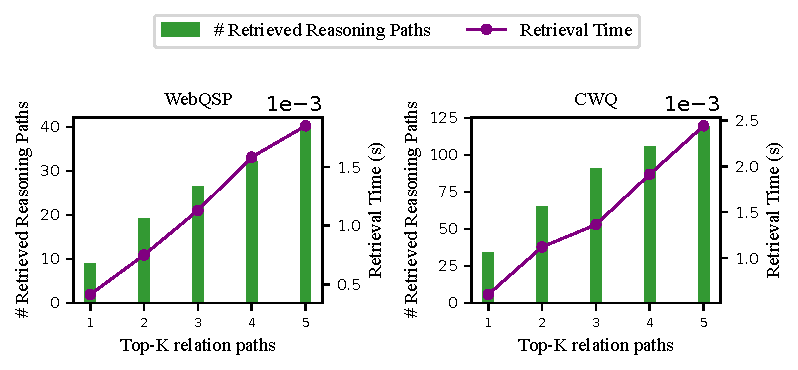
\includegraphics[width=0.8\columnwidth]{images/costs.pdf}
    \end{center}
    \caption{Average retrieval time and average number of retrieved reasoning paths w.r.t. the number of top-$K$ relation paths.}
    \label{fig:retrieval_cost}
\end{figure}

\begin{table}[]
    \centering
    \caption{F1 scores of \ourmethod and its variants for different hops of questions.}
    \label{tab:exp_hops}
    \resizebox{.7\columnwidth}{!}{%
        \begin{tabular}{@{}c|ccc|ccc@{}}
            \toprule
            \multirow{2}{*}{Methods} & \multicolumn{3}{c|}{WebQSP} & \multicolumn{3}{c}{CWQ}                                               \\ \cmidrule(l){2-7}
                                     & 1 hop                       & 2 hop                   & $\geq$ 3 hop & 1 hop & 2 hop & $\geq$ 3 hop \\ \midrule
            \ourmethod               & 77.03                       & 64.86                   & -            & 62.88 & 58.46 & 37.82        \\
            \ourmethod w/o reasoning & 57.06                       & 25.49                   & -            & 17.06 & 34.25 & 17.07        \\
            \ourmethod w/o planning  & 50.33                       & 51.66                   & -            & 31.04 & 33.93 & 23.29        \\ \bottomrule
        \end{tabular}
    }
\end{table}


\subsubsection{Performance on different hops}
We present the performance of \ourmethod and its variants on different hops of questions in \Cref{tab:exp_hops}. From results, we can see that \ourmethod achieves better performance than its variants on different hops of questions, especially questions with more than 3 hops. This demonstrates the importance of relation paths for improving the reasoning performance of LLMs on complex questions.

\subsubsection{Performance on different answer numbers}
We also present the performance of \ourmethod and its variants on questions with different numbers of answers in \Cref{tab:exp_number_ans}. From results, we can see that \ourmethod achieves better performance than its variants on questions with different numbers of answers. Specifically, with the number of answer increasing, the performance of \ourmethod w/o planning decreases significantly due to the lack of knowledge from KGs. Although, \ourmethod w/o reasoning can retrieve more answers to improve the performance. It still is inferior to \ourmethod due to the lack of reasoning ability to remove the noise.
\begin{table}[]
    \centering
    \caption{F1 scores of \ourmethod and its variants for questions with varying numbers of answers.}
    \label{tab:exp_number_ans}
    \resizebox{\columnwidth}{!}{%
        \begin{tabular}{@{}c|cccc|cccc@{}}
            \toprule
            \multirow{2}{*}{Methods} & \multicolumn{4}{c|}{WebQSP} & \multicolumn{4}{c}{CWQ}                                                                                                                               \\ \cmidrule(l){2-9}
                                     & \#Ans = 1                   & 2 $\geq$ \#Ans $\leq$ 4 & 5 $\geq$ \#Ans $\leq$ 9 & \#Ans $\geq$ 10 & \#Ans = 1 & 2 $\geq$ \#Ans $\leq$ 4 & 5 $\geq$ \#Ans $\leq$ 9 & \#Ans $\geq$ 10 \\ \midrule
            \ourmethod               & 67.89                       & 79.39                   & 75.04                   & 58.33           & 56.90     & 53.73                   & 58.36                   & 43.62           \\
            \ourmethod w/o reasoning & 33.49                       & 52.80                   & 58.05                   & 66.01           & 16.61     & 27.06                   & 40.10                   & 34.45           \\
            \ourmethod w/o planning  & 55.03                       & 51.08                   & 44.81                   & 27.00           & 34.08     & 34.16                   & 31.67                   & 25.21           \\ \bottomrule
        \end{tabular}
    }
\end{table}

\subsection{Case Studies: Relation Paths}\label{app:case_rel}
We illustrate several examples of relation paths generated by \ourmethod in \Cref{tab:case_rel}.

\subsection{Case Studies: Interpretable Results}\label{app:case_inter}
We illustrate several examples of interpretable reasoning results generated by \ourmethod in \Cref{tab:case_int}.

\subsection{Prompts}\label{app:prompts}

Planning module aims to generate faithful relation paths as plans for answering the question. The instruction template is presented as follows:

% \LH{Any better way to present the instruction template?}
\begin{minipage}{0.99\columnwidth}
    \centering
    \begin{tcolorbox}[title=Planning Prompt Template]
        \small
        Please generate a valid relation path that can be helpful for answering the following question: \texttt{<Question>}
    \end{tcolorbox}
    \vspace{1mm}
\end{minipage}
where \texttt{<Question>} indicates the question.

The reasoning module takes the question $q$ and a set of reasoning paths $\gW_z$ to generate answers $a$. The instruction template is presented as follows:

\begin{minipage}{0.99\columnwidth}
    \centering
    \begin{tcolorbox}[title=Reasoning Prompt Template]
        \small
        Based on the reasoning paths, please answer the given question. Please keep the answer as simple as possible and return all the possible answers as a list.

        \vspace{10pt}
        Reasoning Paths:

        \texttt{<Reasoning Paths>}

        \vspace{10pt}
        Question:

        \texttt{<Question>}
    \end{tcolorbox}
\end{minipage}

where \texttt{<Reasoning Paths>} denotes the retrieved reasoning paths $\gW_z$ which are formatted as a series of structural sentences:

\begin{minipage}{0.99\columnwidth}
    \centering
    $e_0\to r_1\to e_1\to \dots \to r_l \to e_l$\\
    $\dots$\\
    $e_0\to r_1\to e_1\to \dots \to r_l \to e_l$.
\end{minipage}

To exploit the explanation ability of \ourmethod, we design a new instruction template for the reasoning module to generate interpretable results. The instruction template is presented as follows:

\begin{minipage}{0.99\columnwidth}
    \centering
    \begin{tcolorbox}[title=Explanation Prompt Template]
        \small
        Based on the reasoning paths, please answer the given question and explain why.

        \vspace{10pt}
        Here are some examples:

        \texttt{<Examples>}

        \vspace{10pt}
        Reasoning Paths:

        \texttt{<Reasoning Paths>}

        \vspace{10pt}
        Question:

        \texttt{<Question>}
    \end{tcolorbox}
\end{minipage}

where the $\texttt{Examples}$ denotes a few-shot human-annotated examples to demonstrate the explanation process.

% Please add the following required packages to your document preamble:
% \usepackage{booktabs}
% \usepackage{graphicx}
% \usepackage[table,xcdraw]{xcolor}
% If you use beamer only pass "xcolor=table" option, i.e. \documentclass[xcolor=table]{beamer}
\begin{table}[h]
    \centering
    \caption{Examples of the generated relation paths.}
    \label{tab:case_rel}
    \resizebox{.97\columnwidth}{!}{%
        \begin{tabular}{@{}p{2.5in}|l@{}}
            \toprule
            Question                                                                                                      &
            Top-3 Relation Paths                                                                                            \\\midrule
            what does jamaican people speak?                                                                               &
            \begin{tabular}[c]{@{}l@{}}$z_1:$   location.country.languages\_spoken\\      $z_2:$ language.human\_language.countries\_spoken\_in\\      $z_3:$ location.country.official\_language\end{tabular}                                                                                       \\\midrule
            where is jamarcus russell from?                                                                                &
            \begin{tabular}[c]{@{}l@{}}$z_1:$   location.location.people\_born\_here\\      $z_2:$ people.person.place\_of\_birth\\      $z_3:$ sports.sports\_league\_draft\_pick.player $\to$   sports.sports\_league\_draft\_pick.location\end{tabular}                                                                                       \\ \midrule
            where did edgar allan poe died?                                                                                &
            \begin{tabular}[c]{@{}l@{}}$z_1:$   people.deceased\_person.place\_of\_death\\      $z_2:$ people.cause\_of\_death.people\\      $z_3:$ people.person.place\_of\_birth\end{tabular}                                                                                       \\ \midrule
            what highschool did harper lee go to?                                                                          &
            \begin{tabular}[c]{@{}l@{}}$z_1:$ people.person.education   $\to$ education.educational\_institution.students\_graduates\\      $z_2:$ education.education.student $\to$   education.educational\_institution.students\_graduates\\      $z_3:$ people.person.education $\to$ education.education.institutio\end{tabular}                                                                                       \\ \midrule
            what are the songs that justin bieber   wrote?                                                                 &
            \begin{tabular}[c]{@{}l@{}}$z_1:$   music.recording.artist\\      $z_2:$ music.composition.composer\\      $z_3:$ music.composer.compositions\end{tabular}                                                                                       \\ \midrule
            what are the religions practiced in   indonesia?                                                               &
            \begin{tabular}[c]{@{}l@{}}$z_1:$ people.person.nationality   $\to$ people.person.religion\\      $z_2:$ location.statistical\_region.religions $\to$   location.religion\_percentage.religion\\      $z_3:$ location.country.languages\_spoken $\to$ religion.religion.languages\end{tabular}                                                                                       \\ \midrule
            Lou Seal is the mascot for the team that   last won the World Series when?                                    &
            \begin{tabular}[c]{@{}l@{}}$z_1:$ sports.mascot.team $\to$   sports.sports\_championship\_event.champion\\      $z_2:$ sports.mascot.team $\to$ sports.sports\_team.championships\\      $z_3:$ sports.sports\_championship\_event.championship\end{tabular}                                                                                       \\ \midrule
            % What country in the Caribbean contains Saint Michael Parish? & \begin{tabular}[c]{@{}l@{}}$z_1:$  location.administrative\_division.first\_level\_division\_of\\      $z_2:$ location.location.containedby\\      $z_3:$ location.location.contains\end{tabular} \\ \midrule
            What type of government is used in the   country with Northern District?                                      &
            \begin{tabular}[c]{@{}l@{}}$z_1:$   location.administrative\_division.first\_level\_division\_of $\to$   government.form\_of\_government.countries\\      $z_2:$ location.administrative\_division.first\_level\_division\_of $\to$   location.country.form\_of\_government\\      $z_3:$ administrative\_division.first\_level\_division\_of $\to$   government.form\_of\_government.countries\end{tabular}                                                                                       \\ \midrule
            The people from the country that contains   Nord-Ouest Department speak what languages today?                 &
            \begin{tabular}[c]{@{}l@{}}$z_1:$   location.administrative\_division.first\_level\_division\_of $\to$   language.human\_language.countries\_spoken\_in\\      $z_2:$ location.administrative\_division.first\_level\_division\_of $\to$   location.country.languages\_spoken\\      $z_3:$ base.aareas.schema.administrative\_area.administrative\_parent $\to$   location.country.languages\_spoken\end{tabular}                                                                                       \\ \midrule
            What stadium does the team with mascot   named Hank play at?                                                  &
            \begin{tabular}[c]{@{}l@{}}$z_1:$ sports.mascot.team $\to$   sports.sports\_facility.teams\\      $z_2:$ sports.sports\_team.team\_mascot $\to$   sports.sports\_facility.teams\\      $z_3:$ sports.mascot.team $\to$ sports.sports\_team.arena\_stadium\end{tabular}                                                                                      \\ \midrule
            Which popular sports team in Spain, that   won the 2014 Eurocup Finals championship?                          &
            \begin{tabular}[c]{@{}l@{}}$z_1:$   sports.sports\_team.championships $\to$   sports.sports\_team\_location.teams\\      $z_2:$ sports.sports\_team.location $\to$   sports.sports\_team\_location.teams\\      $z_2:$ sports.sports\_team.location $\to$   sports.sports\_team\_location.teams\\      $z_3:$ sports.sports\_team\_location.teams\end{tabular}                                                                                      \\ \midrule
            What educational institution with the   mascot named Washington University Bear did Tennessee Williams go to? &
            \begin{tabular}[c]{@{}l@{}}$z_1:$   education.educational\_institution.mascot\\      $z_2:$ people.person.nationality $\to$ location.location.containedby\\      $z_3:$ education.education.student $\to$ education.education.institution\end{tabular}\\ \midrule
            Who is the current head coach of the NFL squad owned by the Rooney family? & \begin{tabular}[c]{@{}l@{}}$z_1:$   sports.professional\_sports\_team.owner\_s $\to$ american\_football.football\_coach.current\_team\_head\_coached\\      $z_2:$ sports.professional\_sports\_team.owner\_s $\to$ american\_football.football\_team.current\_head\_coach\\      $z_3:$ american\_football.football\_coach.current\_team\_head\_coached \end{tabular}\\\midrule

            What is the home field of the sports team whose mascot is named Fredbird? & \begin{tabular}[c]{@{}l@{}}$z_1:$   sports.mascot.team $\to$ sports.sports\_facility.teams\\      $z_2:$ sports.sports\_team.team\_mascot $\to$ sports.sports\_facility.teams\\      $z_3:$ sports.mascot.team $\to$ sports.sports\_team.arena\_stadium \end{tabular}\\
            \bottomrule
        \end{tabular}%
    }
\end{table}
\begin{table}[]
    \centering
    \caption{Examples of faithful and interpretable reasoning of \ourmethod.}
    \vspace{-3mm}
    \label{tab:case_int}
    \resizebox{1\columnwidth}{!}{%
    \begin{tabular}{@{}c|p{5in}@{}}
        \toprule
        Question             & Lou Seal is the mascot for the team that last won the World Series when?                                                                                                                                                                                                                                                                                         \\ \midrule
        Answer               & 2014                                                                                                                                                                                                                                                                                                                                                 \\ \midrule
        Reasoning Paths      & Lou Seal $\to$ sports.mascot.team $\to$ San Francisco Giants $\to$ sports.sports\_championship\_event.champion $\to$ 2014 World Series                                                                                                                                                                                        \\
        \midrule
        \ourmethod & \begin{tabular}[c]{@{}p{5in}@{}}Based on the provided reasoning paths, we can determine when the team for which Lou Seal is the mascot last won the World Series:\\\\

            1. Lou Seal is associated with the San Francisco Giants.\\
            2. The San Francisco Giants are associated with winning the 2014 World Series.\\\\
            
            Therefore, the San Francisco Giants, the team for which Lou Seal is the mascot, last won the World Series in 2014.\end{tabular}                                                                                                                                                                                                                                                                                                                                            \\ \bottomrule
            \toprule
            Question             & what is my timezone in louisiana?                                                                                                                                                                                                                                                                                         \\ \midrule
            Answer               & Central Time Zone                                                                                                                                                                                                                                                                                                                                                 \\ \midrule
            Reasoning Paths      & \begin{tabular}[c]{@{}p{5in}@{}} Louisiana $\to$ location.location.partially\_containedby $\to$ Tangipahoa River $\to$ geography.river.origin $\to$ Osyka $\to$ location.location.time\_zones $\to$ Central Time Zone \\\\
                Louisiana $\to$ location.location.containedby $\to$ Alexandria $\to$ location.location.containedby $\to$ United States of America $\to$ location.location.time\_zones $\to$ Central Time Zone 
            \end{tabular}\\
        \midrule
            \ourmethod & \begin{tabular}[c]{@{}p{5in}@{}}Based on the reasoning paths provided, it can be determined that Louisiana is in the Central Time Zone. \\\\

                Here's the explanation: \\\\
                
                1. The first reasoning path tells us that Louisiana is partially contained by the Tangipahoa River, which is a geographical feature. However, it doesn't directly mention the time zone. \\\\
                
                2. The second reasoning path establishes that Louisiana is contained by Alexandria, which is in turn contained by the United States of America. The United States of America is in the Central Time Zone. \\\\
                
                Therefore, based on these reasoning paths, the time zone in Louisiana is the Central Time Zone.\end{tabular}                                                                                                                                                                                                                                                                                                                                            \\ \bottomrule
                \toprule
                Question             & Which child of Walt Disney died from lung cancer?                                                                                                                                                                                                                                                                                         \\ \midrule
                Answer               & Sharon Mae Disney                                                                                                                                                                                                                                                                                                                             \\ \midrule
                Reasoning Paths      & \begin{tabular}[c]{@{}p{5in}@{}} Lung cancer $\to$ people.deceased\_person.cause\_of\_death $\to$ Sharon Mae Disney\\\\
                    Lung cancer $\to$ people.deceased\_person.cause\_of\_death $\to$ Walt Disney \\\\
                    Walt Disney $\to$ people.deceased\_person.cause\_of\_death $\to$ Lung cancer \\\\
                    Walt Disney $\to$ people.person.children $\to$ Diane Disney Miller \\\\
                    Walt Disney $\to$ people.cause\_of\_death.people $\to$ Circulatory collapse \\\\
                    Walt Disney $\to$ people.person.parents $\to$ Flora Call Disney \\\\
                    Walt Disney $\to$ people.person.parents $\to$ Elias Disney \\\\
                    Walt Disney $\to$ people.person.parents $\to$ Sharon Mae Disney
                \end{tabular}\\
            \midrule
                \ourmethod & \begin{tabular}[c]{@{}p{5in}@{}}Based on the reasoning paths provided, it appears that Sharon Mae Disney is the child of Walt Disney who died from lung cancer.\\\\ 
                    
                The reasoning path "Walt Disney $\to$ people.deceased\_person.cause\_of\_death $\to$ Lung cancer" directly connects Walt Disney to lung cancer as a cause of death, and since Sharon Mae Disney is also linked to lung cancer as a cause of death through the path "Lung cancer $\to$ people.deceased\_person.cause\_of\_death $\to$ Sharon Mae Disney," it can be concluded that Sharon Mae Disney is the child of Walt Disney who died from lung cancer.\end{tabular}                                                                                                                                                                                                                                                                                                                                            \\ \bottomrule
    \end{tabular}}
\end{table}